\lhead{\emph{Classifier Trees}}

\chapter{Classifier Trees}
\label{classifier_trees}

Common classifiers described in the Chapter \ref{common_classifiers} return results in form of a class label that provided pattern was classified to. Such approach leaves no room for estimating class-belonging probabilities which, in return, results in inability to reject provided data, treating it as an outlier. By combining those classifiers and organising them in a complex structures it is possible to create objects with unique rejection capabilities in exchange for slightly increased pattern-processing time. This chapter describes such structures, shaped in form of binary trees.

\section{Balanced Tree}

\subsection{Structure}
\label{BalancedTreeStructure}

The main idea behind Balanced Tree structure is to create a graph tree in which every path from root to leaf consists of increasingly precise classifiers. What it means is that every pattern, that should be classified, is tested against certain number of common classifiers, where each subsequent one is clarifying this unknown pattern's affiliation to one of the classes.

The Balanced Tree construction begins with creation of a root node which represents a situation in a classification process in which all possible class memberships for an unknown pattern are taken into account. It can be said that the root of the Balanced Tree represents a set consisting of all classes in the training set, because it is yet unknown from which class a pattern would be. The process of clarifying pattern's class belonging starts by designating the central points for each class in the set of classes represented by this node. This is done by calculating arithmetic average of all points from certain class set: \[ p_{central} = \frac{\sum\limits_{i=1}^n p_{i}}{n} \] where $n$ is number of elements $p_{i}$ belonging to certain class in the dataset. Next step involves using clustering algorithm to divide all of those central points into two distinctive sets. The idea is to group those class representatives that are most similar to each other. The process of Balanced Tree structure creation is continued further by passing two classes sets designated by clustering algorithm, one to each child nodes. The process of new node creation is then applied to each of those two child nodes and continued until there is only one class left. A node representing only one class cannot use clustering method because there is insufficient number of classes to divide, and so it becomes the tree leaf. 

\begin{figure}[htp]
	\centering
	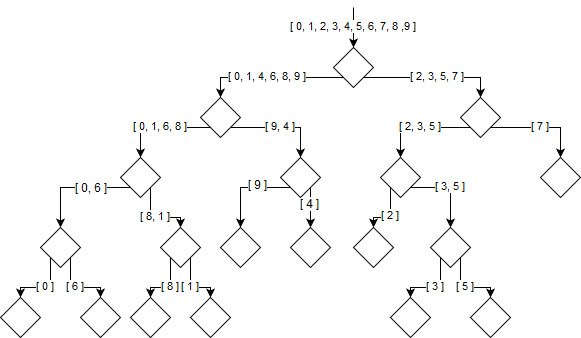
\includegraphics[width=0.8\textwidth]{Figures/balanced_tree_structure.jpg}
	\caption{Balanced Tree structure obtained during real life tests}
	\label{balanced_tree_structure}\vspace{-3pt}
\end{figure}

\subsection{Classifiers creation}

After finishing Balanced Tree architecture creation each non-leaf node is assigned a binary classifier trained on a data consisting of a training samples from classes assigned to this particular node. Those classes that are represented by its left child node are joined together and treated as a class '0', while the ones in the right child node are labelled as a class '1'. For example, if there are four classes assigned to a certain tree node, labelled as $a, b, c, d$, and a clustering method divided them into two sets $a, d$ (assigned to left child node) and $b, c$ (assigned to right child node), the classifier will be trained on data samples treating points from classes $a, d$ as if they all were from an artificial class '0' and classes $b, c$ as class '1'. The only issue that arises from such attitude is inability for leaf nodes to have their own classifiers. This is due to leafs being the last nodes in a tree, having no child nodes. To circumvent this shortcoming a solution is proposed that treats leaf node as if it had left child with the same assigned class as a parent, and a right child with assigned every existing class in the training dataset except for the class assigned to its sibling (left child node).

\subsection{Classification rules}

When an unknown, new pattern is presented to the Balanced Tree, it traverses a path from a root to a leaf node in order to be classified or rejected. This path strongly depends on classifiers in each node and their classification decision. As it was described earlier each node is assigned certain number of classes that it represents. The main task of each node's classifier is to decide if the provided pattern belongs to internal class '0' or '1'. In other words it tries to determine to which set of classes this unknown elements is most similar to. After decision is taken the patterns is sent further to the left child node in case it was classified as '0' or right one if classified as '1'. Each subsequent classifier is more precise and better clarifies pattern's class affiliation. After reaching leaf node the final classification test is made. The classifier in a leaf node is trained in an one-versus-all manner. If the unknown element is recognized as a member of a class assigned to this particular leaf, it is finally labelled as an element from that class. On the other hand if it is classified as a "rest" pattern, it gets rejected. The scheme for this approach can be seen on Figure \ref{balanced_tree_rejection}. Rejection relies on the assumption that if the pattern traversed path all way down to the leaf node, while being sent to next nodes basing on increasingly strict classifiers' decisions, and ends up being recognized as a point from outside of most probable class (the one assigned to the leaf node), then it probably is not similar enough to any class from the training set.

\begin{figure}[htp]
	\centering
	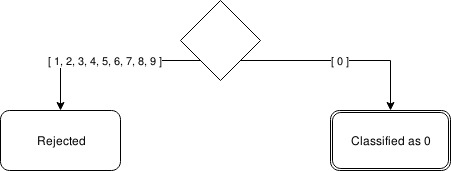
\includegraphics[width=0.6\textwidth]{Figures/balanced_tree_rejection.jpg}
	\caption{Balanced Tree rejection scheme in leaf node}
	\label{balanced_tree_rejection}\vspace{-3pt}
\end{figure}

\subsection{Implementation details}

Creation of Balanced Tree structure starts from tree root and is done recursively. Each node, that is not a tree leaf, is assigned certain set of classes which is a subset of all classes in a tree (root node is assigned all). The next step involves clustering method dividing node's class set into two disjoint sets. This procedure is done on 'class central points' which are average points of all elements in each class. Clustering algorithm divides those points thus providing two new sets for both child nodes. After that node trains its classifier on data set consisting of two classes created by taking all elements from training data for left and right child nodes' classes sets. The node-creation procedure is then applied for both node's children. The leaf creation algorithm is slightly different as it does not need usage of clustering. Classifier is trained on data set created from combining elements from training data that belongs to the same class the leaf node represents (those points' new class is labelled '0') and elements from every other class (which are labelled '1')\label{balanced_tree:one-vs-rest}. To ensure that both '0' and '1' classes have the same number of entries the '1' class set must be trimmed. This is done at its creation step by taking less elements from each class in order to have the same number (or nearly identical) of elements overall in the whole set, e.g. having training data set consisting of ten classes labelled from '0' to '9', with total of 10,000 elements, set '0' for leaf representing class '2' will have 1,000 entries of elements from class '2' taken from training data and set '1' will have 999 elements in total but will consist of elements from classes '0', '1', '3', '4', '5', '6', '7', '8', '9' taken from training data with 111 elements from each class.

\section{Slanting Tree}

\label{slanting_tree_description}

\subsection{Structure}

The Slanting Tree structure differs greatly from Balanced Tree's one. The concept implemented in Slanting Tree assumes that the unknown pattern, that is sent for classification, should be iteratively compared against each class representatives. Only when it is similar enough to points from certain class, more precise tests are made that ensure its affiliation. Should the tests fail, the pattern continues its iteration over other classes as if wasn't ever supposed to belong to this class. Rejection occurs when every test fails.

Construction of the Slanting Tree is fairly simple, unlike the Balanced Tree. Each node represents exactly one class. Nodes are chained together in such manner that when traversing Slanting Tree from the root to the last node by choosing always the left child, exactly one node for each class in the training set is visited. Each of these nodes has also a right child that can be treated as a node between its parent and its parent's left child, that extends the path received when going from root to the last node by taking always the left node's successor. Each right child node represents the same class from the training data set as its parent does.

\subsection{Classifiers creation}

Each tree node in Slanting Tree has its own binary classifier, trained in a 'one-versus-rest' manner. Training is done on data containing two classes, where the first one consists of patterns from the training set which belong to the same class as the node represents, and the second one is obtained by concatenating patterns of each class from the training set except for the class represented by the node. To prevent the situation in which node and its right child have the classifier trained on the same data (because both nodes represent the same class) certain changes to training patterns must be introduced. This ensures that every classifier in the Slanting Tree is unique and can be used during classification procedure.


\subsection{Classification rules}

The classification starts from the root node, where the unknown pattern is tested by the first classifier and has its class affiliation checked. If the obtained result indicates that it isn't similar to the class represented by this node (gets classified as an element from the 'rest' class), the classification process is continued in the next node, which is the left child of the current one. If the opposite situation occurs, and the classifier accepts presented pattern as a representative of current node's class, the process is repeated in the right child node which uses more strict classifier. This is done to ensure that the unknown element, which is supposedly from the certain class, really belongs to it. If this test fails, the pattern is sent to the node as if the previous test also failed (it is sent to the left child of the current node's parent). In case of success the pattern gets successfully classified. When all tests fail (there is no more nodes to send pattern to) the element gets rejected.

\subsection{Implementation details}

\label{slanting_tree_implementation}Creation of Slanting Tree is done recursively, starting from the root node. All classes that should be distinguishable by this tree structure are sorted by their labels and stored in an array object. This object is later used during node creation method to check what classes have already been covered by previous nodes. Every non-leaf node represents only one native class and has its binary classifier trained in 'one-vs-rest' manner, the same way the tree leafs' classifiers in Balanced Tree are (see \ref{balanced_tree:one-vs-rest}). The next step involves creating left child node for the next native class in the array object that has not yet been used. In case of no classes left the function returns without creating new node. The last step consists of right child creation, which is a leaf node. Leafs in a Slanting Tree represent the same native classes their parent node did, but their classifiers, although built using same 'one-vs-rest' approach, are trained on a different data sets in order to create more accurate results. Usually trained classifier does not achieve 100\% accuracy even on a training test that was used during its creation. There are some samples from first class that get classified as elements from the second and vice versa. Such mistakes can help determine what kind of corrections can be made to the classifier. For every non-leaf node, after its classifier training, there's set of elements from the first class that were correctly recognized (those are the elements from the class this particular node is representing) and set of elements from the second class that were mistakenly recognized as elements from the first class. Those two sets are used in this node's child leaf node's classifier creation. Of course before training those two sets must be the same size, ideally having the same number of elements as two sets used in parent's classifier training. For each missing element in either of sets the new object is generated by randomly selecting one element from this set and applying normal distribution (with standard deviation 1) to all of its features in a feature vector, thus getting new sample that can be added to the set. In case of having less than certain number of elements (implementation checks for 10 or less elements) in either of sets before new point generation algorithm takes place, those sets are filled with randomly selected points from parent node's classifier training sets.

\begin{figure}[htp]
	\centering
	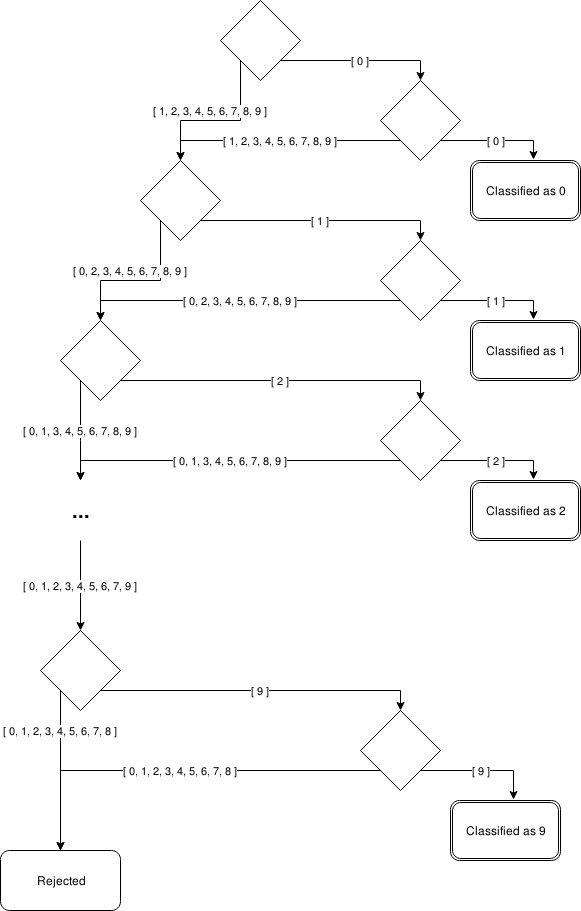
\includegraphics[width=0.7\textwidth]{Figures/slanting_tree_structure.jpg}
	\caption{Bottom part of the Slanting Tree with nodes for classes 8 and 9 (nodes for classes from 0 - 7 not visible).}
	\label{fig:rejection_version2}\vspace{-3pt}
\end{figure}

\section{Slanting Tree with ordered classes}

\subsection{Description}

The basic Slanting Tree structure assigns classes to its nodes based on an arbitrary, lexicographic order. This approach leaves its implementation vulnerable to situation in which label changes occur. Slanting Tree with ordered classes tries to circumvent this disadvantage by sorting classes without the need to know their labels, based on their spatial relations. Every set of points belonging to certain class in a training dataset can be transformed into one point, being the centre of that particular class. Next the distance to every other centre point in the training dataset is calculated for each class centre, and only the lowest value is saved. The new class order is based on those values, which are sorted in the descending order.

\subsection{Implementation details}

Steps required to build Slanting Tree with ordered classes are mostly the same as in \ref{slanting_tree_implementation}. Instead of creating nodes for classes using their lexicographic order, the ordering technique described in the previous Section is used. During computations only one point, called the class central point, for each class in the training dataset is used. Those are calculated the same way as in \ref{BalancedTreeStructure}, by getting the average value of all training patterns from one class. Sorted class labels are used further during classifier tree creation process the same way as in original Slanting Tree.

\section{Slanting Tree 2}

\subsection{Description}

Much like previously described Slanting Tree, this one has its nodes arranged in the same architecture. The difference lies in leaf nodes which, unlike the original Slanting Tree, are not using modified training data sets and use different classifier types instead (e.g. parent nodes using SVM classifier and their right children nodes using random forest). The idea behind this implementation relies on the assumption that various classifiers tend to wrongly classify different patterns, so when combining them rejection rate as well as classification rate should be vastly improved. Other than that there are no further changes and everything described in the Section \ref{slanting_tree_description} applies to Slanting Tree 2.

\subsection{Implementation details}

Creation procedure is mostly the same as in \ref{slanting_tree_implementation}. The only differences are present in nodes creation method where instead of creating new training patterns for the right child node, different classifier type is trained on the same data from the parent node.

\section{Results}

Described in this chapter classifier trees were tested with various common classifiers: SVM, kNN and random forest, using different parameters. Over 500 tests were held. Results in form of quality measurements (see Chapter \ref{quality_measures}) for training, test and letters sets were gathered in form of two matrices with 12 rows and 10 columns, one for training and one for test data. Each row in the matrix corresponds to one of the quality evaluation measurements, and each column represents value of corresponding measurement scored by certain classifier tree using one of the common classifiers. See Table \ref{example_result_matrix} for reference.

\begin{table}[htp]
	\centering
	\caption{Example empty result matrix}
	\label{example_result_matrix}
	\resizebox{\textwidth}{!}{
	\begin{tabular}{l|l|l|l|l|l|l|l|l|l|}
		\cline{2-10}
		\textbf{}                                                & \multicolumn{3}{l|}{\textbf{Balanced Tree}} & \multicolumn{3}{l|}{\textbf{Slanting Tree}} & \multicolumn{3}{l|}{\textbf{Slanting Tree 2}} \\ \cline{2-10} 
		\textbf{}                                                & \textbf{kNN}  & \textbf{SVM}  & \textbf{RF} & \textbf{kNN}  & \textbf{SVM}  & \textbf{RF} & \textbf{kNN}   & \textbf{SVM}  & \textbf{RF}  \\ \hline
		\multicolumn{1}{|l|}{\textbf{Strict Acc.}}           &               &               &             &               &               &             &                &               &              \\ \hline
		\multicolumn{1}{|l|}{\textbf{Fine Acc.}}             &               &               &             &               &               &             &                &               &              \\ \hline
		\multicolumn{1}{|l|}{\textbf{Strict Native Sens.}} &               &               &             &               &               &             &                &               &              \\ \hline
		\multicolumn{1}{|l|}{\textbf{Acc.}}                  &               &               &             &               &               &             &                &               &              \\ \hline
		\multicolumn{1}{|l|}{\textbf{Native Prec.}}          &               &               &             &               &               &             &                &               &              \\ \hline
		\multicolumn{1}{|l|}{\textbf{Native Sens.}}        &               &               &             &               &               &             &                &               &              \\ \hline
		\multicolumn{1}{|l|}{\textbf{Native F-measure}}          &               &               &             &               &               &             &                &               &              \\ \hline
		\multicolumn{1}{|l|}{\textbf{Foreign Prec.}}         &               &               &             &               &               &             &                &               &              \\ \hline
		\multicolumn{1}{|l|}{\textbf{Foreign Sens.}}       &               &               &             &               &               &             &                &               &              \\ \hline
		\multicolumn{1}{|l|}{\textbf{Foreign F-measure}}         &               &               &             &               &               &             &                &               &              \\ \hline
	\end{tabular}
	}
\end{table}

Every common classifier that was used by any of tree nodes was tested with different parameters. SVM had its C, gamma and kernel options adjusted (see Chapter \ref{common_classifiers} for every parameter explanation). Values were as follows \[ C: [ 1, 2, 4, 8, 16 ] \] \[ gamma: [ 2^{-1}, 2^{-2}, 2^{-3}, 2^{-4} ] \]  \[ kernel: [ rbf, poly ] \] 
Adjustments for kNN were made for only one parameter, using euclidean metrics \[ n\_neighbors: [ 3, 5, 7, 10 ] \]
Random forests also had modifications applied to one parameter \[ n\_estimators: [ 30, 50, 100, 150 ] \]
When evaluating results quality evaluation measurements were taken into account (see Chapter \ref{quality_measures}). In the next few subsections there is short summary for each classifier tree using different internal classifiers. Because the results obtained for Slanting Tree with ordered classes were almost exactly the same as for regular Slanting Tree (with arbitrary class order) the results tables do not include scores achieved for the original Slanting Tree (without computed order of classes) to maintain their clarity.

\begin{table}[htp]
	\centering
	\caption{Measures values (described in Chapter \ref{quality_measures}) for classifier trees using various common classifiers on training data (described in Chapter \ref{datasets})}
	\label{classifier_trees_training_results}
	\resizebox{\textwidth}{!}{
	\begin{tabular}{l|l|l|l|l|l|l|l|l|l|}
		\cline{2-10}
		\textbf{}                                                & \multicolumn{3}{l|}{\textbf{Balanced Tree}}   & \multicolumn{3}{l|}{\textbf{Slanting Tree}} & \multicolumn{3}{l|}{\textbf{Slanting Tree 2}} \\ \cline{2-10} 
		\textbf{}                                                & \textbf{kNN}     & \textbf{SVM} & \textbf{RF} & \textbf{kNN}  & \textbf{SVM}  & \textbf{RF} & \textbf{kNN}   & \textbf{SVM}  & \textbf{RF}  \\ \hline
		\multicolumn{1}{|l|}{\textbf{Strict Acc.}}           & 20.67 & 44.92        & 41.47       & 22.76         & 29.70         & 50.29       & 38.34          & 41.51         & 40.59        \\ \hline
		\multicolumn{1}{|l|}{\textbf{Fine Acc.}}             & 92.66 & 99.33        & 100.00      & 90.61         & 91.79         & 92.43       & 94.08          & 95.41         & 95.94        \\ \hline
		\multicolumn{1}{|l|}{\textbf{Strict Native Sens.}} & 92.64 & 99.09        & 100.00      & 90.00         & 91.73         & 92.43       & 93.06          & 95.26         & 95.79        \\ \hline
		\multicolumn{1}{|l|}{\textbf{Acc.}}                  & 22.21 & 45.06        & 41.47       & 24.72         & 31.42         & 51.88       & 39.57          & 42.47         & 41.44        \\ \hline
		\multicolumn{1}{|l|}{\textbf{Native Prec.}}          & 21.23 & 27.60        & 26.38       & 21.70         & 23.41         & 30.35       & 25.62          & 26.69         & 26.35        \\ \hline
		\multicolumn{1}{|l|}{\textbf{Native Sens.}}        & 99.99 & 99.76        & 100.00      & 99.33         & 99.93         & 100.00      & 98.91          & 99.84         & 99.84        \\ \hline
		\multicolumn{1}{|l|}{\textbf{Native F-measure}}          & 35.02 & 43.23        & 41.74       & 35.62         & 37.93         & 46.57       & 40.70          & 42.13         & 41.69        \\ \hline
		\multicolumn{1}{|l|}{\textbf{Foreign Prec.}}         & 99.76 & 99.79        & 100.00      & 96.51         & 99.86         & 100.00      & 98.81          & 99.85         & 99.84        \\ \hline
		\multicolumn{1}{|l|}{\textbf{Foreign Sens.}}       & 1.58 & 30.55        & 25.94       & 4.92          & 13.25         & 39.11       & 23.82          & 27.25         & 25.94        \\ \hline
		\multicolumn{1}{|l|}{\textbf{Foreign F-measure}}         & 3.10  & 46.78        & 41.20       & 9.37          & 23.39         & 56.23       & 38.39          & 42.82         & 41.18        \\ \hline
	\end{tabular}
	}
\end{table}

\begin{table}[htp]
	\centering
	\caption{Measures values (described in Chapter \ref{quality_measures}) for classifier trees using various common classifiers on test data (described in Chapter \ref{datasets})}
	\label{classifier_trees_test_results}
	\resizebox{\textwidth}{!}{
		\begin{tabular}{l|l|l|l|l|l|l|l|l|l|}
			\cline{2-10}
			\textbf{}                                                & \multicolumn{3}{l|}{\textbf{Balanced Tree}} & \multicolumn{3}{l|}{\textbf{Slanting Tree}} & \multicolumn{3}{l|}{\textbf{Slanting Tree 2}} \\ \cline{2-10} 
			\textbf{}                                                & \textbf{kNN}  & \textbf{SVM}  & \textbf{RF} & \textbf{kNN}  & \textbf{SVM}  & \textbf{RF} & \textbf{kNN}   & \textbf{SVM}  & \textbf{RF}  \\ \hline
			\multicolumn{1}{|l|}{\textbf{Strict Acc.}}           & 10.79         & 37.04         & 32.81       & 13.41         & 21.18         & 44.21       & 30.72          & 33.94         & 32.75        \\ \hline
			\multicolumn{1}{|l|}{\textbf{Fine Acc.}}             & 91.86         & 96.44         & 95.56       & 88.89         & 91.49         & 90.36       & 93.45          & 95.02         & 94.56        \\ \hline
			\multicolumn{1}{|l|}{\textbf{Strict Native Sens.}} & 91.77         & 94.03         & 93.23       & 88.00         & 90.97         & 89.03       & 91.33          & 92.80         & 92.67        \\ \hline
			\multicolumn{1}{|l|}{\textbf{Acc.}}                  & 11.62         & 37.39         & 33.26       & 14.53         & 22.05         & 45.18       & 31.37          & 34.44         & 33.30        \\ \hline
			\multicolumn{1}{|l|}{\textbf{Native Prec.}}          & 10.35         & 13.77         & 13.03       & 10.59         & 11.53         & 15.54       & 12.73          & 13.24         & 13.08        \\ \hline
			\multicolumn{1}{|l|}{\textbf{Native Sens.}}        & 99.90         & 97.50         & 97.57       & 99.00         & 99.43         & 98.53       & 97.73          & 97.67         & 98.00        \\ \hline
			\multicolumn{1}{|l|}{\textbf{Native F-measure}}          & 18.75         & 24.13         & 22.99       & 19.13         & 20.66         & 26.85       & 22.53          & 23.33         & 23.08        \\ \hline
			\multicolumn{1}{|l|}{\textbf{Foreign Prec.}}         & 99.28         & 99.08         & 98.94       & 97.74         & 99.52         & 99.58       & 98.93          & 99.04         & 99.13        \\ \hline
			\multicolumn{1}{|l|}{\textbf{Foreign Sens.}}       & 1.58          & 30.55         & 25.94       & 4.92          & 13.25         & 39.11       & 23.82          & 27.25         & 25.94        \\ \hline
			\multicolumn{1}{|l|}{\textbf{Foreign F-measure}}         & 3.10          & 46.70         & 41.11       & 9.38          & 23.38         & 56.16       & 38.40          & 42.74         & 41.12        \\ \hline
		\end{tabular}
	}
\end{table}

Results gathered in Table \ref{classifier_trees_training_results} and Table \ref{classifier_trees_test_results} prove that combining commonly used classifiers by putting them in more complex structures does not affect overall classification capabilities. Of course the quality of determining patterns' affiliations relies mostly on the type of the classifier used, but is also affected by classifier's parameters and the tree structure. 

Trees using SVM classifier yield better results when using radial basis function (rbf) kernel along with C parameter set to 16 and $\gamma$ to 0.5. During calculations it was observed that the $\gamma$ parameter didn't have as much impact on final results, unlike the C parameter which, when decreasing its value, lowered achieved scores. For Slanting Tree 2 the SVM classifier performed best when paired up with Random Forest which may indicate that both of those classifiers tend to misclassifying different patterns (hence better rejection option rates).

Using Random Forest classifier yields different scores depending on which tree structure is used. Whereas Balanced Tree performs best when using Random Forest with 30 estimators, both Slanting Tree and Slanting Tree 2 get better results while utilizing classifier with 100 estimators. Interesting may be the fact that the best performing Slanting Tree 2 uses Random Forest combined with SVM classifiers with the exactly same parameters' values as when using SVM classifier backed up by Random Forest one. In both cases results are very similar which proves that those classifiers tend to cooperate well.

Unfortunately, among all classifiers tested, the kNN one performs the worst when used in all of the three trees. While this doesn't mean that the classifications rates were very low, in fact the differences between scores achieved by using kNN and SVM or Random Forest were negligible, rejection option was almost non-existent. The best results, achieved by Slanting Tree 2, were obtained when using Random Forest as a second classifier. All results for kNN classifier for each of classifier tree described in this chapter, presented in the tables, were achieved when using $n\_neighbors$ parameter value of 10.

\section{Summary}

All of the classifier trees introduced in this chapter had good classification capabilities, very similar to the plain common classifiers they used. It is worth noting that not only did the classification rate stayed the same, but also rejection capabilities were introduced. Among all classifiers combinations tested it was the Slanting tree using random forests with 100 estimators that performed the best. Tables \ref{classifier_trees_training_results} and \ref{classifier_trees_test_results} show score achieved by this tree structure. Although being the best, classification rate achieved by this particular Slanting Tree may not be considered good, as it's lower than 50\%. At best it could be seen as mediocre. Despite trying different classifiers and their parameters combinations no better solution could be found while using tree structures described in this chapter. The final conclusion can be made that the classifier trees introduced in this paper do not perform well enough to be used as a valid rejection mechanism. While still maintaining high classification rates those structures are slower than other popular classifiers which questions their usefulness.